\documentclass[tikz,border=5pt]{standalone}

\usepackage{graphicx}
\usepackage{tikz}
\usetikzlibrary{positioning}
\usepackage{comment}


\usepackage[scaled]{helvet}
\renewcommand{\familydefault}{\sfdefault}

\begin{document}
\begin{tikzpicture}[
  node distance = 1cm and 1.5cm,
  font=\sffamily,
  every node/.style={inner sep=0, outer sep=0}
]

%--- Top row: Ground truth
\node (plot-gt) {};
\node[right=4.3cm of plot-gt] (plot-gt2) {};
\node[right=4.3cm of plot-gt2] (plot-gt3) {};
%\node[above=1.3cm of plot-gt] {\ \ \ \ \ \ \ \ \ \ \ \ \ \ \ \ \ \ \ \ \ \ \ \ \ \ \ \ \ \ \ \ \ \ \ \ \ \ $\sqrt{\mathcal{J}(\theta)}$};
\node[above=1.7cm of plot-gt, xshift=2cm](FI){Fisher Information (FI)};
\node[left=0.5cm of FI, yshift=-0.0cm](label-a){\large a};
\node[right=0cm of plot-gt] {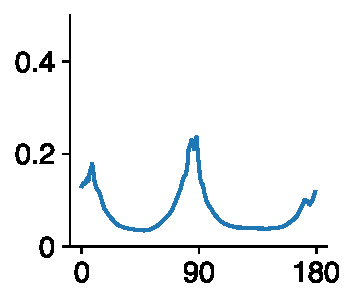
\includegraphics[width=0.32\textwidth]{figures/RunGardelle_FreePrior_CosineLoss_Downsampled_TargetSize_VIZ_OnlyEncoding.py_8_0-21_10.0_180_1000_1.pdf}};
\node[right=0cm of plot-gt] {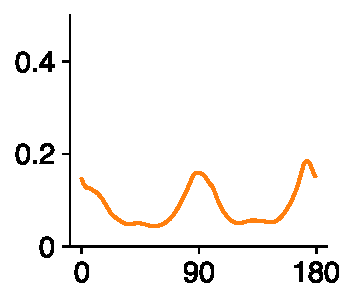
\includegraphics[width=0.32\textwidth]{figures/RunGardelle_FreePrior_CosineLoss_Downsampled_TargetSize_VIZ_OnlyEncoding.py_8_0-21_10.0_180_1000_2.pdf}};
\node[right=0cm of plot-gt] {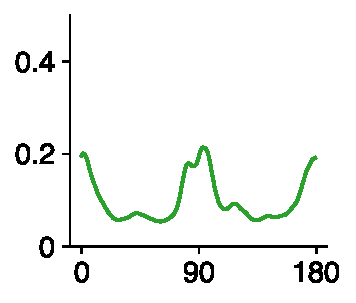
\includegraphics[width=0.32\textwidth]{figures/RunGardelle_FreePrior_CosineLoss_Downsampled_TargetSize_VIZ_OnlyEncoding.py_8_0-21_10.0_180_1000_3.pdf}};
\node[right=0cm of plot-gt] {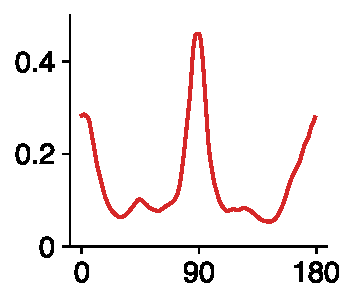
\includegraphics[width=0.32\textwidth]{figures/RunGardelle_FreePrior_CosineLoss_Downsampled_TargetSize_VIZ_OnlyEncoding.py_8_0-21_10.0_180_1000_4.pdf}};
\node[right=0cm of plot-gt] {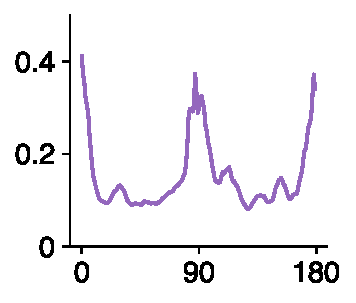
\includegraphics[width=0.32\textwidth]{figures/RunGardelle_FreePrior_CosineLoss_Downsampled_TargetSize_VIZ_OnlyEncoding.py_8_0-21_10.0_180_1000_5.pdf}};

%\node[above=1.3cm of plot-gt2] {\ \ \ \ \ \ \ \ \ \ \ \ \ \ \ \ \ \ \ \ \ \ \ \ \ \ \ \ \ \ \ \ \ \ \ \ \ \ $F'(\theta)$};
\node[above=1.7cm of plot-gt2, xshift=0.5cm] {\ \ \ \ \ \ \ \ \ \ \ \ \ \ \ \ \ \ \ \ \ \ \ \ \ \ \  \ \ \ \ \ \ \ \ \ Normalized FI};
\node[right=4.7cm of label-a, yshift=-0.0cm](label-b){\large b};
\node[right=0.0cm of plot-gt2] {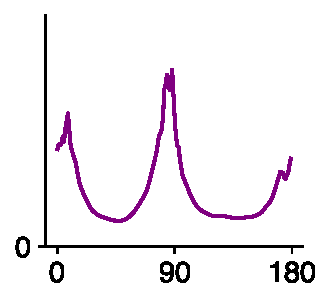
\includegraphics[width=0.32\textwidth]{figures/RunGardelle_FreePrior_CosineLoss_Downsampled_TargetSize_VIZ_OnlyEncodingNorm.py_8_0-21_10.0_180_1000_1.pdf}};
\node[right=0.0cm of plot-gt2] {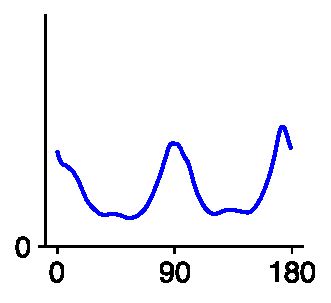
\includegraphics[width=0.32\textwidth]{figures/RunGardelle_FreePrior_CosineLoss_Downsampled_TargetSize_VIZ_OnlyEncodingNorm.py_8_0-21_10.0_180_1000_2.pdf}};
\node[right=0.0cm of plot-gt2] {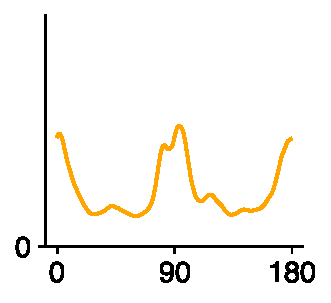
\includegraphics[width=0.32\textwidth]{figures/RunGardelle_FreePrior_CosineLoss_Downsampled_TargetSize_VIZ_OnlyEncodingNorm.py_8_0-21_10.0_180_1000_3.pdf}};
\node[right=0.0cm of plot-gt2] {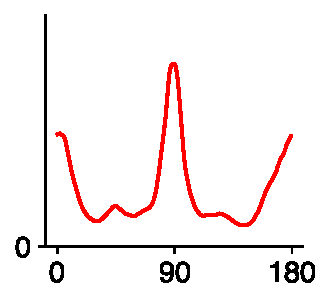
\includegraphics[width=0.32\textwidth]{figures/RunGardelle_FreePrior_CosineLoss_Downsampled_TargetSize_VIZ_OnlyEncodingNorm.py_8_0-21_10.0_180_1000_4.pdf}};
\node[right=0.0cm of plot-gt2] {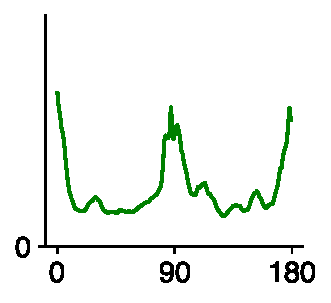
\includegraphics[width=0.32\textwidth]{figures/RunGardelle_FreePrior_CosineLoss_Downsampled_TargetSize_VIZ_OnlyEncodingNorm.py_8_0-21_10.0_180_1000_5.pdf}};

%\node[above=1.3cm of plot-gt3] {\ \ \ \ \ \ \ \ \ \ \ \ \ \ \ \ \ \ \ \ \ \ \ \ \ \ \ \ \ \ \ \ \ \ \ \ \ \ $\int\sqrt{\mathcal{J}(\theta)}d\theta$};
\node[above=1.7cm of plot-gt3, xshift=0.5cm] {\ \ \ \ \ \ \ \ \ \ \ \ \ \ \ \ \ \ \ \ \ \ \  \ \ \ \ \ \ \ \ \ \ \ \ \ \ Total FI};
\node[right=3.9cm of label-b, yshift=-0.0cm](label-c){\large c};
\node[right=0.0cm of plot-gt3] {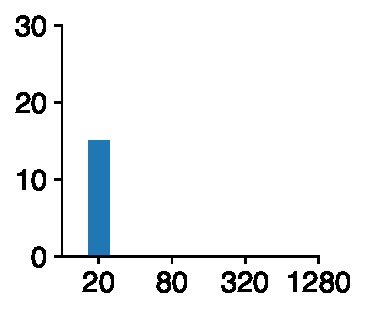
\includegraphics[width=0.32\textwidth]{figures/RunGardelle_FreePrior_CosineLoss_Downsampled_TargetSize_VIZ_OnlyEncodingTotalFI.py_8_0-21_10.0_180_1000_1.pdf}};
\node[right=0.0cm of plot-gt3] {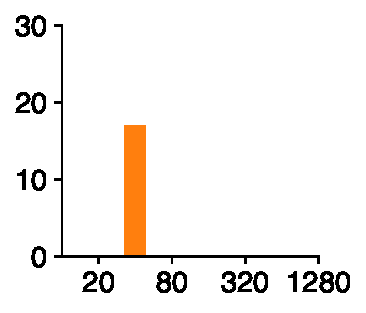
\includegraphics[width=0.32\textwidth]{figures/RunGardelle_FreePrior_CosineLoss_Downsampled_TargetSize_VIZ_OnlyEncodingTotalFI.py_8_0-21_10.0_180_1000_2.pdf}};
\node[right=0.0cm of plot-gt3] {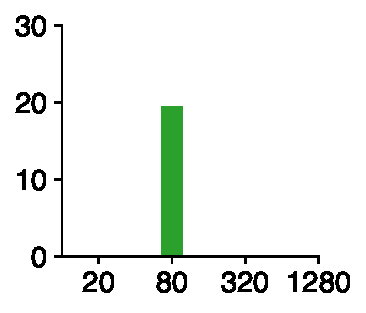
\includegraphics[width=0.32\textwidth]{figures/RunGardelle_FreePrior_CosineLoss_Downsampled_TargetSize_VIZ_OnlyEncodingTotalFI.py_8_0-21_10.0_180_1000_3.pdf}};
\node[right=0.0cm of plot-gt3] {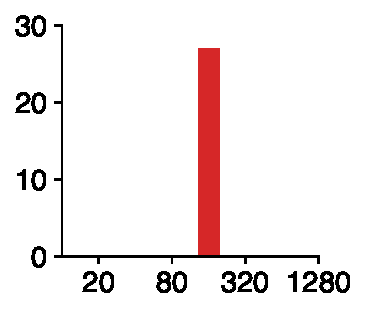
\includegraphics[width=0.32\textwidth]{figures/RunGardelle_FreePrior_CosineLoss_Downsampled_TargetSize_VIZ_OnlyEncodingTotalFI.py_8_0-21_10.0_180_1000_4.pdf}};
\node[right=0.0cm of plot-gt3] {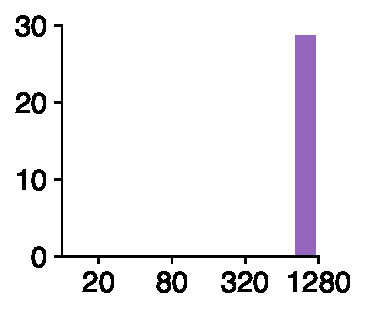
\includegraphics[width=0.32\textwidth]{figures/RunGardelle_FreePrior_CosineLoss_Downsampled_TargetSize_VIZ_OnlyEncodingTotalFI.py_8_0-21_10.0_180_1000_5.pdf}};



\node[
  anchor=north west,   % align the label’s top-left corner
  xshift=-2mm,         % move 2mm left  (into the plot)
  yshift= 15mm          % move 2mm up    (into the plot)
] at (plot-gt.south east) {\scriptsize [1/deg]};



\node[
  anchor=north west,   % align the label’s top-left corner
  xshift=38mm,         % move 2mm left  (into the plot)
  yshift= -12mm          % move 2mm up    (into the plot)
] at (plot-gt.south east) {\scriptsize [deg]};



\node[
  anchor=north west,   % align the label’s top-left corner
  xshift=38mm,         % move 2mm left  (into the plot)
  yshift= -12mm          % move 2mm up    (into the plot)
] at (plot-gt3.south east) {\scriptsize [ms]};




\begin{comment}
python3 RunGardelle_FreePrior_CosineLoss_Downsampled_TargetSize_VIZ_OnlyEncoding.py 8 0 10.0 180 1 1000 21
python3 RunGardelle_FreePrior_CosineLoss_Downsampled_TargetSize_VIZ_OnlyEncoding.py 8 0 10.0 180 2 1000 21
python3 RunGardelle_FreePrior_CosineLoss_Downsampled_TargetSize_VIZ_OnlyEncoding.py 8 0 10.0 180 3 1000 21
python3 RunGardelle_FreePrior_CosineLoss_Downsampled_TargetSize_VIZ_OnlyEncoding.py 8 0 10.0 180 4 1000 21
python3 RunGardelle_FreePrior_CosineLoss_Downsampled_TargetSize_VIZ_OnlyEncoding.py 8 0 10.0 180 5 1000 21

python3 RunGardelle_FreePrior_CosineLoss_Downsampled_TargetSize_VIZ_OnlyEncodingNorm.py 8 0 10.0 180 1 1000 21
python3 RunGardelle_FreePrior_CosineLoss_Downsampled_TargetSize_VIZ_OnlyEncodingNorm.py 8 0 10.0 180 2 1000 21
python3 RunGardelle_FreePrior_CosineLoss_Downsampled_TargetSize_VIZ_OnlyEncodingNorm.py 8 0 10.0 180 3 1000 21
python3 RunGardelle_FreePrior_CosineLoss_Downsampled_TargetSize_VIZ_OnlyEncodingNorm.py 8 0 10.0 180 4 1000 21
python3 RunGardelle_FreePrior_CosineLoss_Downsampled_TargetSize_VIZ_OnlyEncodingNorm.py 8 0 10.0 180 5 1000 21

python3 RunGardelle_FreePrior_CosineLoss_Downsampled_TargetSize_VIZ_OnlyEncodingTotalFI.py 8 0 10.0 180 1 1000 21
python3 RunGardelle_FreePrior_CosineLoss_Downsampled_TargetSize_VIZ_OnlyEncodingTotalFI.py 8 0 10.0 180 2 1000 21
python3 RunGardelle_FreePrior_CosineLoss_Downsampled_TargetSize_VIZ_OnlyEncodingTotalFI.py 8 0 10.0 180 3 1000 21
python3 RunGardelle_FreePrior_CosineLoss_Downsampled_TargetSize_VIZ_OnlyEncodingTotalFI.py 8 0 10.0 180 4 1000 21
python3 RunGardelle_FreePrior_CosineLoss_Downsampled_TargetSize_VIZ_OnlyEncodingTotalFI.py 8 0 10.0 180 5 1000 21


\end{comment}

\end{tikzpicture}
\end{document}
